
\documentclass[border=10pt, 12pt]{standalone}
\usepackage[svgnames]{xcolor}
\usepackage{amsmath}
\usepackage{pgfplots}
\pgfplotsset{compat=newest}
\usepackage[sfdefault]{FiraSans}
\usepackage{FiraMono}
\renewcommand*\familydefault{\sfdefault}
\begin{document}
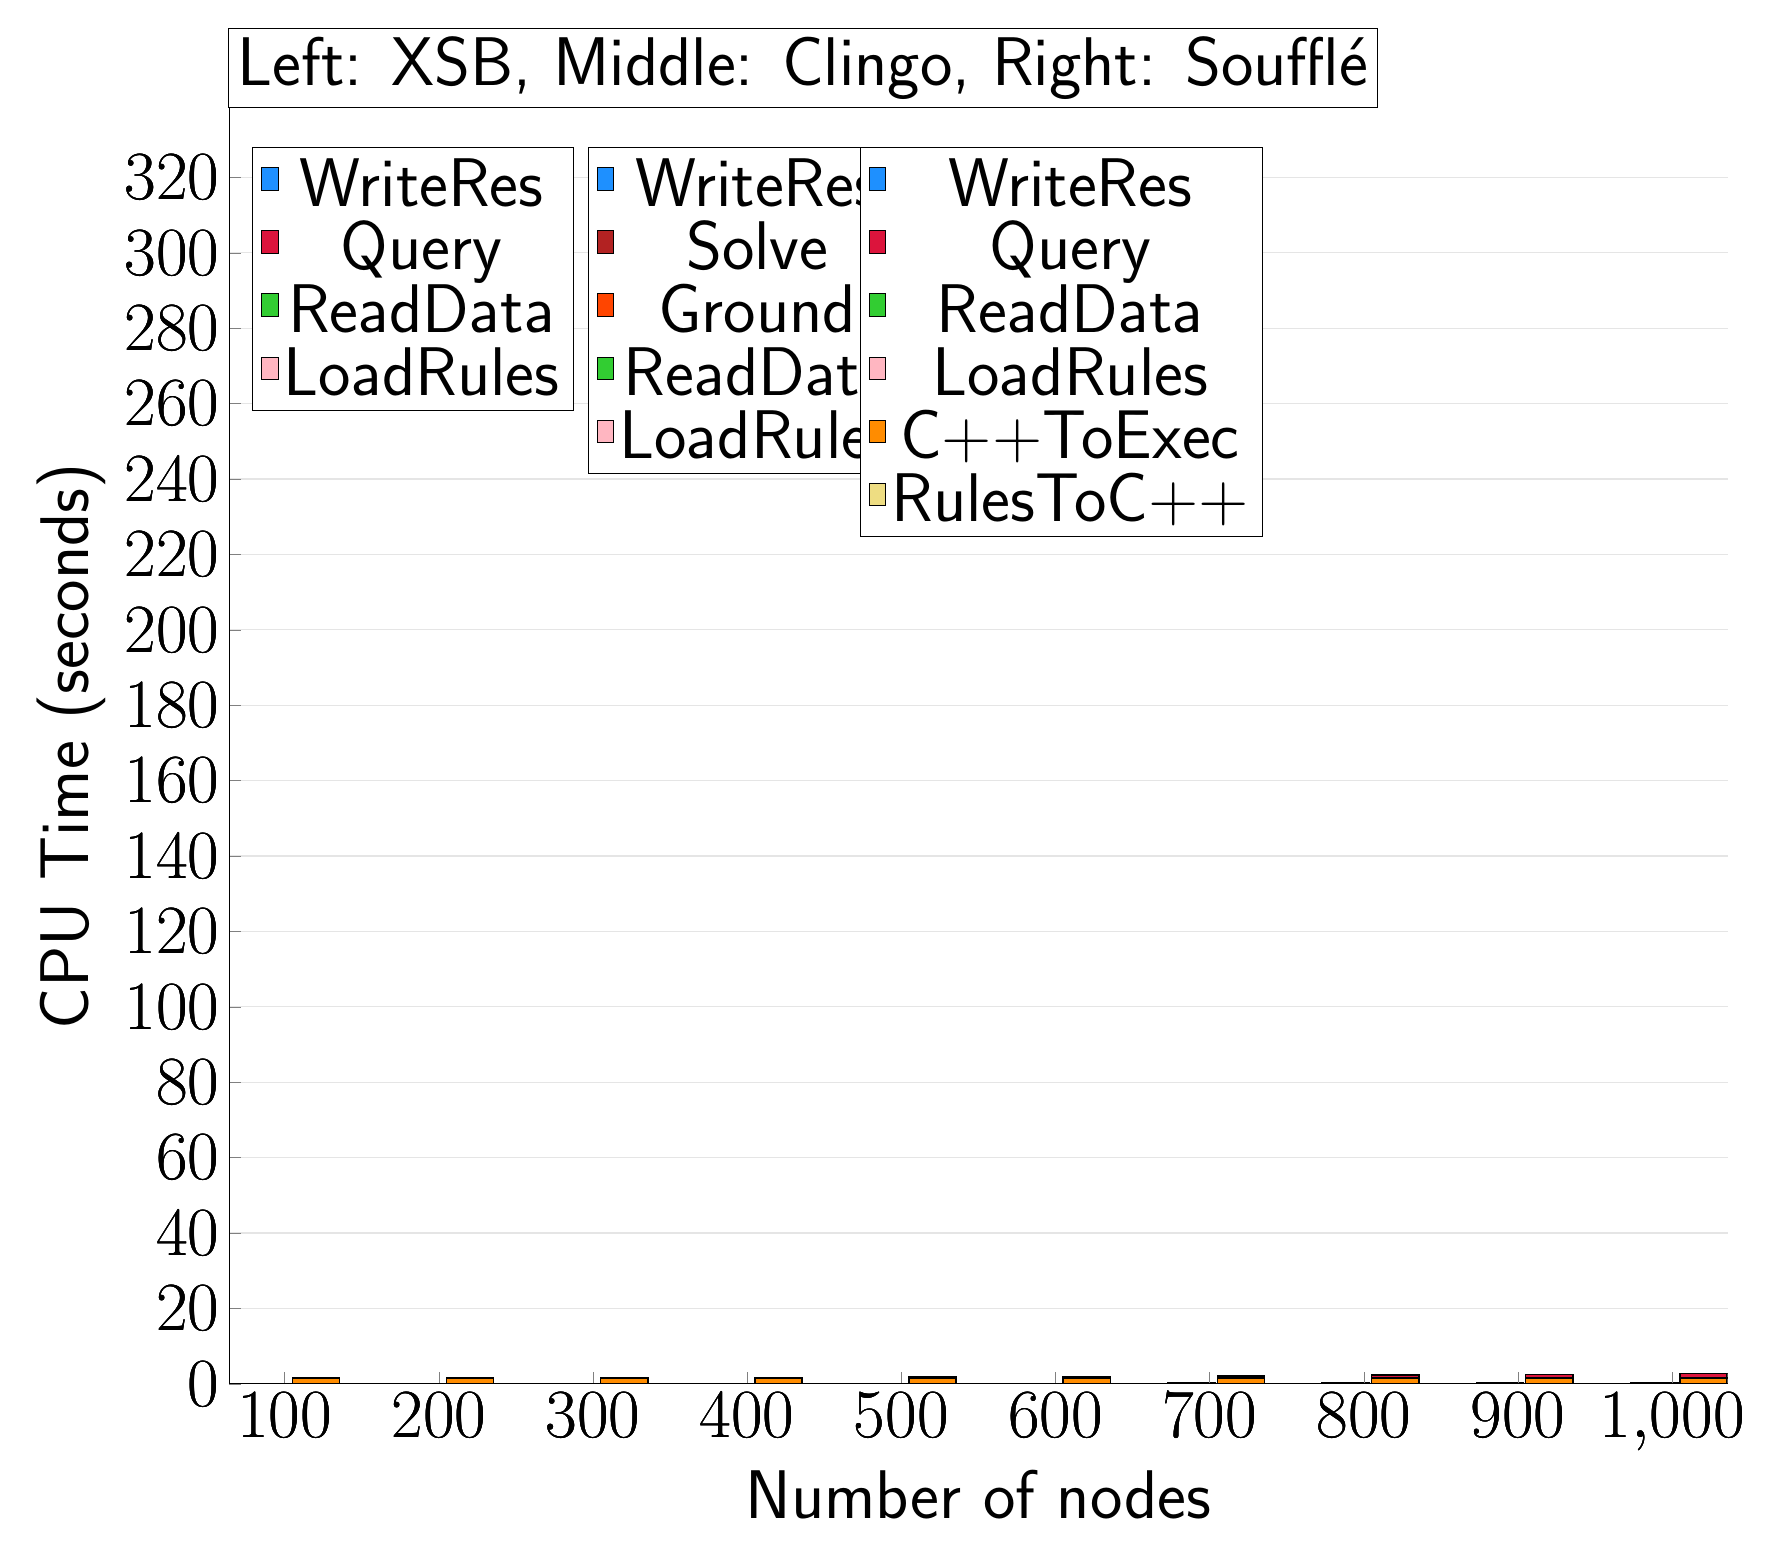
\begin{tikzpicture}
                        \begin{axis}[bar shift=-24.3pt, 
   ybar stacked,
   width=1.7\textwidth,
   bar width=0.6cm,
   ymajorgrids, tick align=inside,
   major grid style={draw=gray!20},
   xtick=data,
   ymin=0, ymax=338.29920000000004,
   axis x line*=bottom,
   axis y line*=left,
   enlarge x limits=0.04,
   legend style={
       at={(0.23, 0.97)},
       anchor=north east,
       legend columns=1,
       font=\Huge,
   },
   ylabel={CPU Time (seconds)},
   xlabel={Number of nodes},
   label style={font=\Huge},
   tick label style={font=\Huge},
]
\addlegendimage{fill=DodgerBlue, draw=black, line width=0.2pt}
\addlegendentry{WriteRes}
\addlegendimage{fill=Crimson, draw=black, line width=0.2pt}
\addlegendentry{Query}
\addlegendimage{fill=LimeGreen, draw=black, line width=0.2pt}
\addlegendentry{ReadData}
\addlegendimage{fill=LightPink, draw=black, line width=0.2pt}
\addlegendentry{LoadRules}
\addplot +[fill=LightPink, draw=black, line width=0.55pt] coordinates {
(100, 0.0005501999999999998)
(200, 0.0005548000000000006)
(300, 0.0005647999999999997)
(400, 0.0005724000000000005)
(500, 0.0005530000000000002)
(600, 0.0005488000000000002)
(700, 0.0005540000000000001)
(800, 0.0005499999999999997)
(900, 0.0005488000000000007)
(1000, 0.0005599999999999998)
};
\addplot +[fill=LimeGreen, draw=black, line width=0.55pt] coordinates {
(100, 0.0001984000000000004)
(200, 0.0002752000000000004)
(300, 0.00048660000000000006)
(400, 0.00043699999999999935)
(500, 0.0005161999999999995)
(600, 0.0005944)
(700, 0.0006684000000000001)
(800, 0.0007540000000000001)
(900, 0.0008249999999999993)
(1000, 0.0009072000000000004)
};
\addplot +[fill=Crimson, draw=black, line width=0.55pt] coordinates {
(100, 1.5799999999999862e-05)
(200, 2.379999999999952e-05)
(300, 3.339999999999974e-05)
(400, 4.220000000000024e-05)
(500, 4.980000000000018e-05)
(600, 5.9999999999999615e-05)
(700, 6.739999999999981e-05)
(800, 7.759999999999953e-05)
(900, 8.400000000000001e-05)
(1000, 8.879999999999931e-05)
};
\addplot +[fill=DodgerBlue, draw=black, line width=0.55pt] coordinates {
(100, 9.099999999999973e-05)
(200, 0.00012399999999999987)
(300, 0.00015139999999999961)
(400, 0.00019339999999999977)
(500, 0.00021620000000000002)
(600, 0.000247600000000001)
(700, 0.0002830000000000006)
(800, 0.00030420000000000067)
(900, 0.0003380000000000005)
(1000, 0.00036260000000000014)
};
\end{axis}

\begin{axis}[bar shift=-6.5pt, 
   ybar stacked,
   width=1.7\textwidth,
   bar width=0.6cm,
   ymajorgrids, tick align=inside,
   major grid style={draw=none},
   xtick=data,
   ymin=0, ymax=338.29920000000004,
   axis x line*=none,
   axis y line*=none,
   enlarge x limits=0.04,
   legend style={
       at={(0.454, 0.97)},
       anchor=north east,
       legend columns=1,
       font=\Huge,
   },
   label style={font=\Huge},
   tick label style={font=\Huge},
]
\addlegendimage{fill=DodgerBlue, draw=black, line width=0.2pt}
\addlegendentry{WriteRes}
\addlegendimage{fill=FireBrick, draw=black, line width=0.2pt}
\addlegendentry{Solve}
\addlegendimage{fill=OrangeRed, draw=black, line width=0.2pt}
\addlegendentry{Ground}
\addlegendimage{fill=LimeGreen, draw=black, line width=0.2pt}
\addlegendentry{ReadData}
\addlegendimage{fill=LightPink, draw=black, line width=0.2pt}
\addlegendentry{LoadRules}
\addplot +[fill=LightPink, draw=black, line width=0.55pt] coordinates {
(100, 0.0)
(200, 0.0)
(300, 0.0)
(400, 0.0)
(500, 0.0)
(600, 0.0)
(700, 0.0)
(800, 0.0)
(900, 0.0)
(1000, 0.0)
};
\addplot +[fill=LimeGreen, draw=black, line width=0.55pt] coordinates {
(100, 0.0)
(200, 0.0)
(300, 0.0)
(400, 0.0)
(500, 0.0)
(600, 0.0)
(700, 0.0)
(800, 0.0)
(900, 0.0)
(1000, 0.0)
};
\addplot +[fill=OrangeRed, draw=black, line width=0.55pt] coordinates {
(100, 0.0)
(200, 0.010000000000000009)
(300, 0.030000000000000027)
(400, 0.055999999999999994)
(500, 0.09000000000000002)
(600, 0.13)
(700, 0.184)
(800, 0.23399999999999999)
(900, 0.30000000000000004)
(1000, 0.384)
};
\addplot +[fill=FireBrick, draw=black, line width=0.55pt] coordinates {
(100, 0.0)
(200, 0.0)
(300, 0.0)
(400, 0.0)
(500, 0.0020000000000000018)
(600, 0.0020000000000000018)
(700, 0.0040000000000000036)
(800, 0.003999999999999981)
(900, 0.0040000000000000036)
(1000, 0.010000000000000007)
};
\addplot +[fill=DodgerBlue, draw=black, line width=0.55pt] coordinates {
(100, 0.0)
(200, 0.0)
(300, 0.0)
(400, 0.0)
(500, 0.0040000000000000036)
(600, -0.0020000000000000018)
(700, -0.0020000000000000018)
(800, -0.003999999999999981)
(900, -0.0040000000000000036)
(1000, -0.010000000000000007)
};
\end{axis}

\begin{axis}[bar shift=11.3pt, 
   ybar stacked,
   width=1.7\textwidth,
   bar width=0.6cm,
   ymajorgrids, tick align=inside,
   major grid style={draw=none},
   xtick=data,
   ymin=0, ymax=338.29920000000004,
   axis x line*=none,
   axis y line*=none,
   enlarge x limits=0.04,
   legend style={
       at={(0.69, 0.97)},
       anchor=north east,
       legend columns=1,
       font=\Huge,
   },
   label style={font=\Huge},
   tick label style={font=\Huge},
]
\addlegendimage{fill=DodgerBlue, draw=black, line width=0.2pt}
\addlegendentry{WriteRes}
\addlegendimage{fill=Crimson, draw=black, line width=0.2pt}
\addlegendentry{Query}
\addlegendimage{fill=LimeGreen, draw=black, line width=0.2pt}
\addlegendentry{ReadData}
\addlegendimage{fill=LightPink, draw=black, line width=0.2pt}
\addlegendentry{LoadRules}
\addlegendimage{fill=DarkOrange, draw=black, line width=0.2pt}
\addlegendentry{C++ToExec}
\addlegendimage{fill=LightGoldenrod, draw=black, line width=0.2pt}
\addlegendentry{RulesToC++}
\addplot +[fill=LightGoldenrod, draw=black, line width=0.55pt] coordinates {
(100, 0.0)
(200, 0.010000000000000002)
(300, 0.0020000000000000005)
(400, 0.006000000000000001)
(500, 0.004000000000000001)
(600, 0.010000000000000002)
(700, 0.008000000000000002)
(800, 0.010000000000000002)
(900, 0.004000000000000001)
(1000, 0.010000000000000002)
};
\addplot +[fill=DarkOrange, draw=black, line width=0.55pt] coordinates {
(100, 1.5240000000000002)
(200, 1.524)
(300, 1.532)
(400, 1.516)
(500, 1.52)
(600, 1.5119999999999998)
(700, 1.518)
(800, 1.5079999999999998)
(900, 1.518)
(1000, 1.51)
};
\addplot +[fill=LightPink, draw=black, line width=0.55pt] coordinates {
(100, 0.000151)
(200, 0.00014780000000000001)
(300, 0.00014800000000000002)
(400, 0.0001408)
(500, 0.00014560000000000002)
(600, 0.00010460000000000001)
(700, 0.0001402)
(800, 0.00013099999999999999)
(900, 0.00013739999999999998)
(1000, 0.0001602)
};
\addplot +[fill=LimeGreen, draw=black, line width=0.55pt] coordinates {
(100, 0.0008552000000000001)
(200, 0.001242)
(300, 0.0015164)
(400, 0.0019316)
(500, 0.0022638000000000003)
(600, 0.0022876)
(700, 0.0030514)
(800, 0.0029618)
(900, 0.0037606000000000002)
(1000, 0.004076000000000001)
};
\addplot +[fill=Crimson, draw=black, line width=0.55pt] coordinates {
(100, 0.0209554)
(200, 0.06425600000000001)
(300, 0.11915040000000002)
(400, 0.20050819999999997)
(500, 0.3086022)
(600, 0.4391328)
(700, 0.6013835999999999)
(800, 0.793763)
(900, 1.0096500000000002)
(1000, 1.260128)
};
\addplot +[fill=DodgerBlue, draw=black, line width=0.55pt] coordinates {
(100, 0.0002736)
(200, 0.0002464)
(300, 0.00021979999999999998)
(400, 0.0002636)
(500, 0.00026940000000000004)
(600, 0.0002934)
(700, 0.000289)
(800, 0.00031800000000000003)
(900, 0.00034619999999999996)
(1000, 0.0003562)
};
\end{axis}


\node[anchor=south, draw, fill=white] at (rel axis cs:0.42,1) {\Huge Left: XSB, Middle: Clingo, Right: Soufflé};
\end{tikzpicture}
\end{document}
                    